\section{Opis działania i obsługi aplikacji}
    \subsection{Przewodnik}

        \subsubsection{Strona internetowa}
            Aplikacja znajduję się na zewnętrznym serwerze VPS i można ją przetestować bez uruchamiana jej na swoim komputerze, dostępna jest pod adresem:
            \begin{itemize}
                \item \url{https://projekt.hu1.pl/}
            \end{itemize}

            \begin{figure}[!htb]
                \centering
                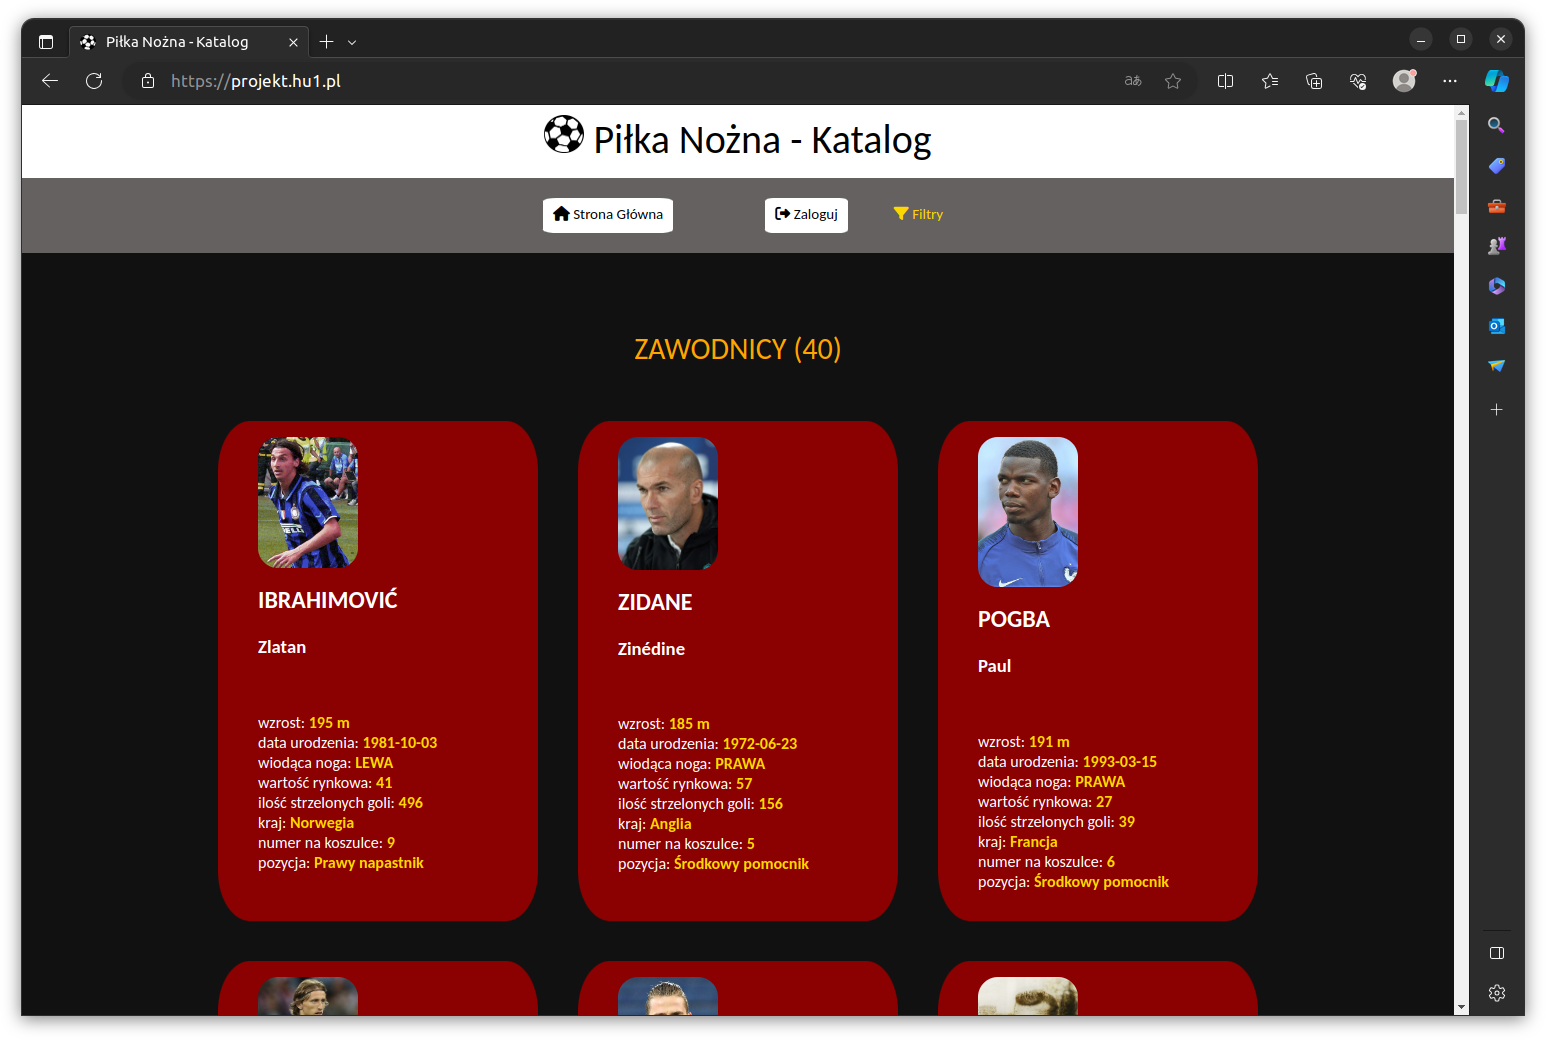
\includegraphics[width=0.6\textwidth]{przewodnik/home.png}
                \caption{Strona Główna}                
            \end{figure}
    
        \subsection{Wyświetlanie oraz filtrowanie piłkarzy}
        
        \subsection{Panel Logowania}
            Panel logowania dostępny jest pod adresem:
            \begin{itemize}
                \item \url{https://projekt.hu1.pl/zaloguj}
            \end{itemize}

            Dane do logowania: 
            \begin{itemize}
                \item Użytkownik: \textbf{admin}
                \item Hasło: \textbf{admin}
            \end{itemize}

                \begin{figure}[!htb]
                    \centering
                    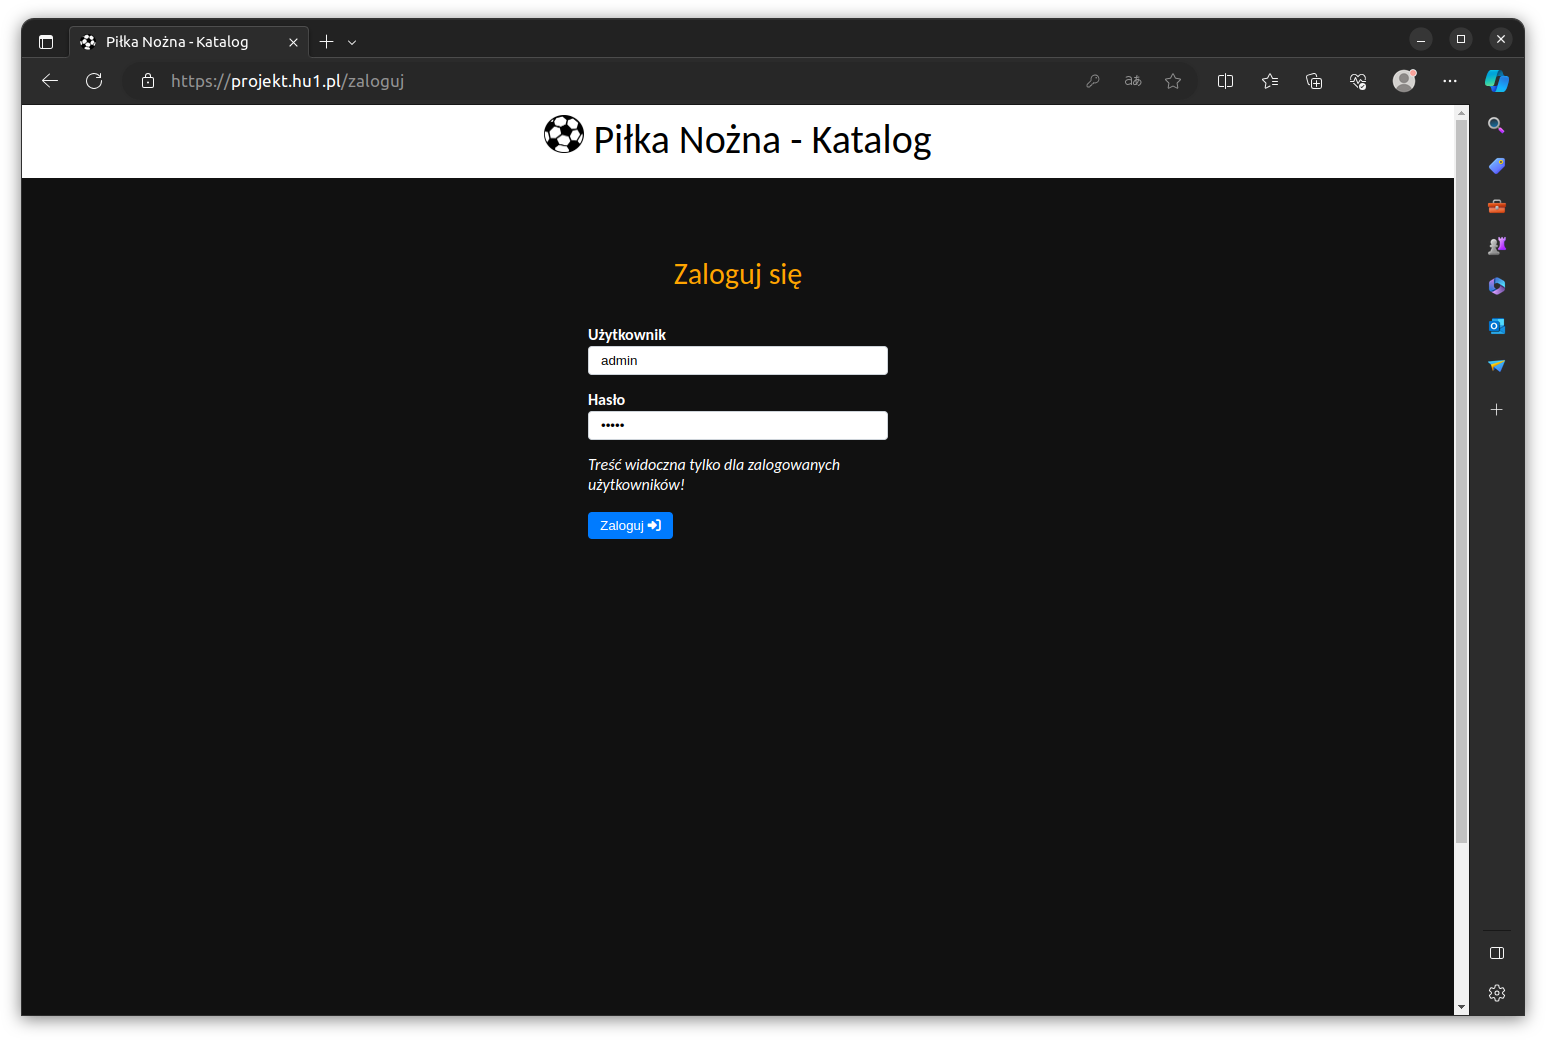
\includegraphics[width=0.6\textwidth]{przewodnik/login.png}
                    \caption{Panel logowania}                
                \end{figure}

        \pagebreak

        \subsection{Panel Administracyjny}
            Jako administrator użytkownik ma podniesione uprawienia i dodatkową zakładkę \textit{Dodaj} oraz przycisk \textit{Edytuj} lub \textit{Usuń} nad zdjęciem piłkarza.

            \begin{figure}[!htb]
                \centering
                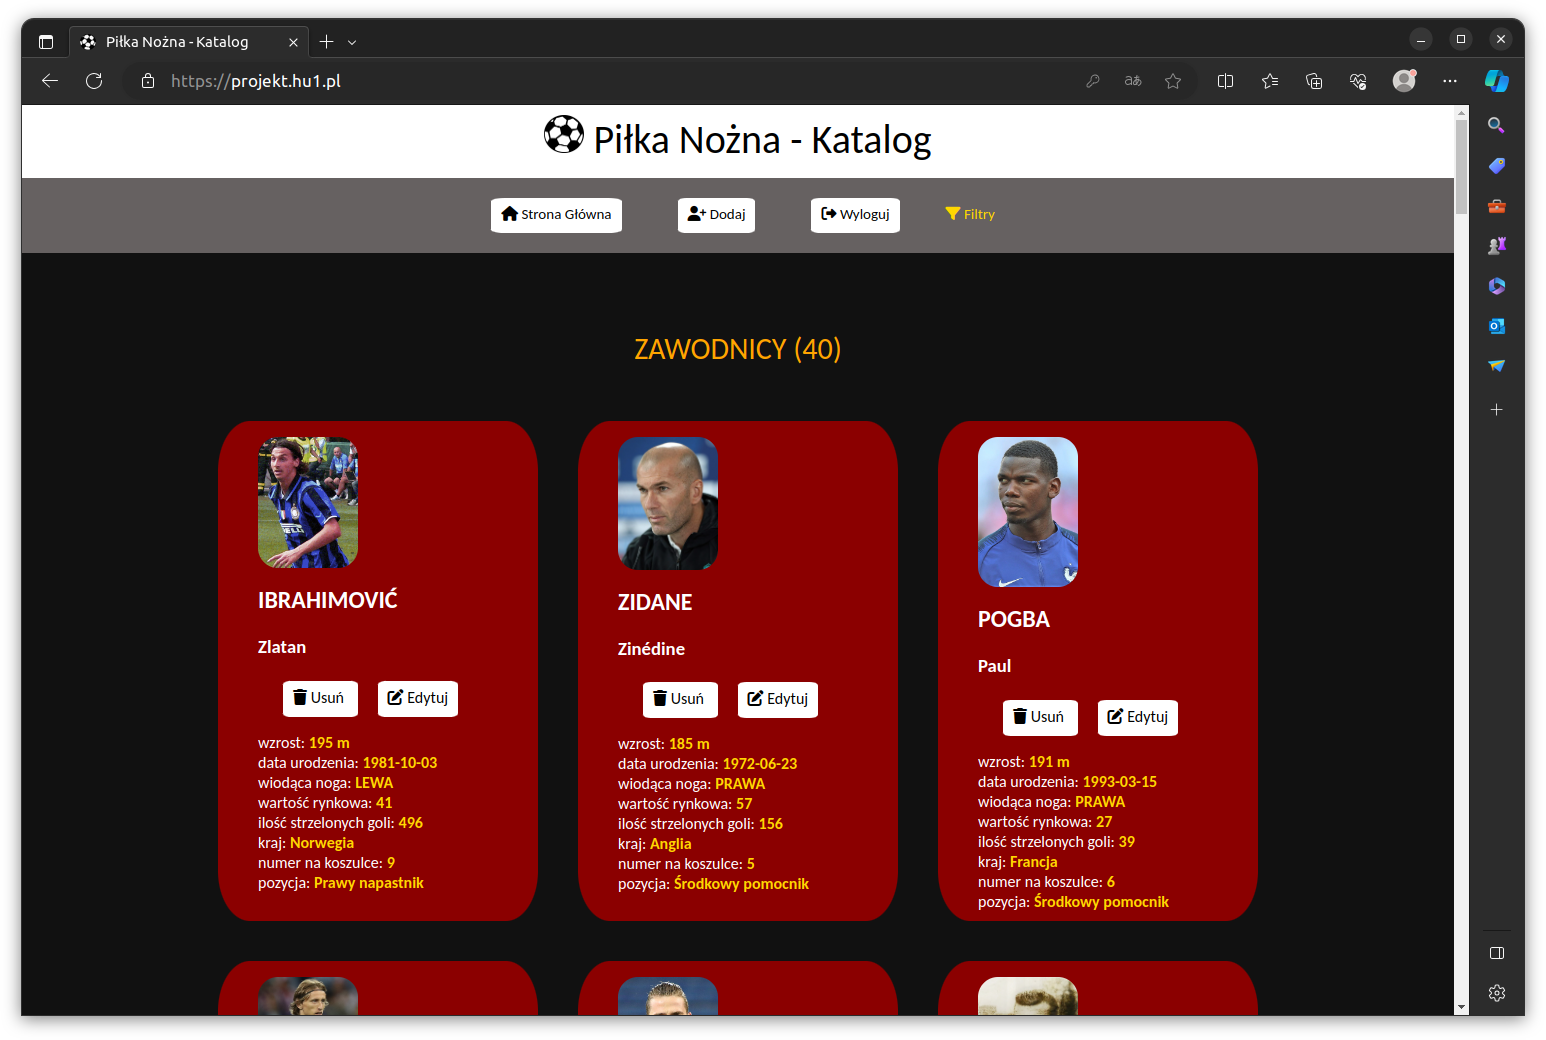
\includegraphics[width=0.6\textwidth]{przewodnik/admin.png}
                \caption{Panel Administracyjny}                
            \end{figure}

        \subsection{Modyfikowanie danych na temat piłkarzy}
                \subsubsection{Dodawanie piłkarza}
                 Na podstawie \textbf{Imienia} oraz \textbf{Nazwiska} zdjęcie piłkarza jest pobierane z serwisu Wikipedia, jeżeli piłkarz ma tam swój artykuł wraz ze zdjęciem (w 90 \% przypadkach posiada), w innym wypadku ustawia domyślne zdjęcie anonimowego użytkownika. 

                    \begin{figure}[!htb]
                        \centering
                        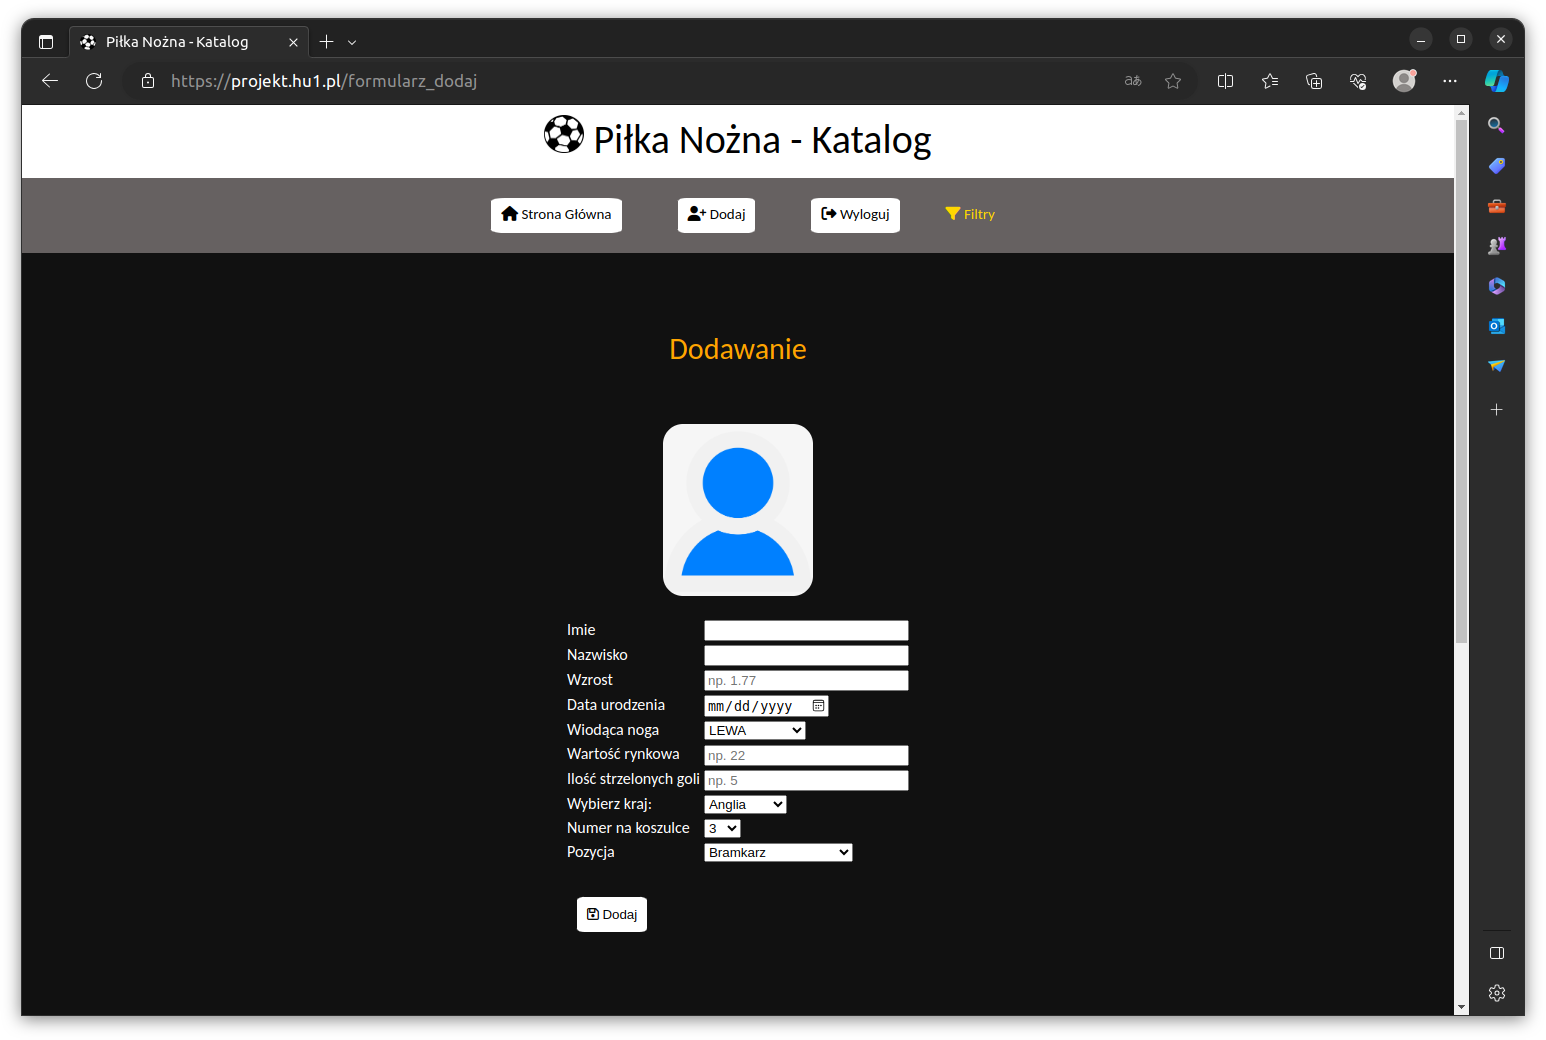
\includegraphics[width=0.6\textwidth]{przewodnik/dodaj.png}
                        \caption{Formularz, który umożliwia dodanie nowego Piłkarza}                
                    \end{figure}
    
                \subsubsection{Usuwanie piłkarza}
                    \begin{figure}[!htb]
                        \centering
                        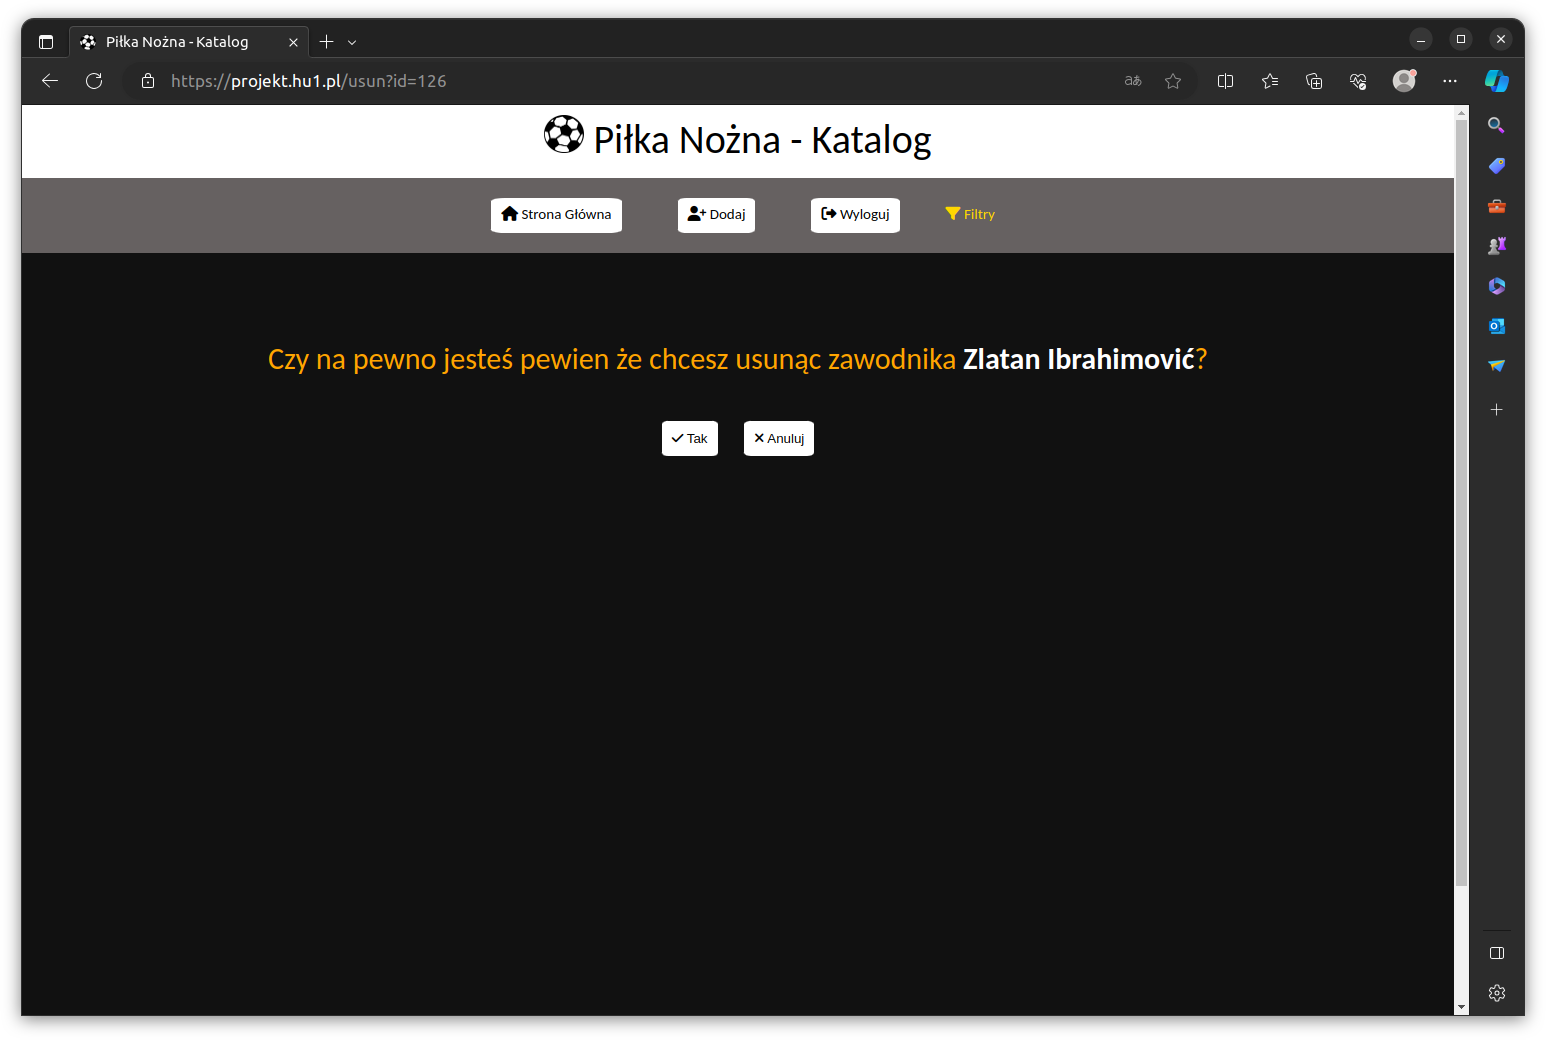
\includegraphics[width=0.6\textwidth]{przewodnik/usun.png}
                        \caption{Potwierdzenie usunięcia Piłkarza}                
                    \end{figure}

                \subsubsection{Edycja piłkarza}

                    \begin{figure}[!htb]
                        \centering
                        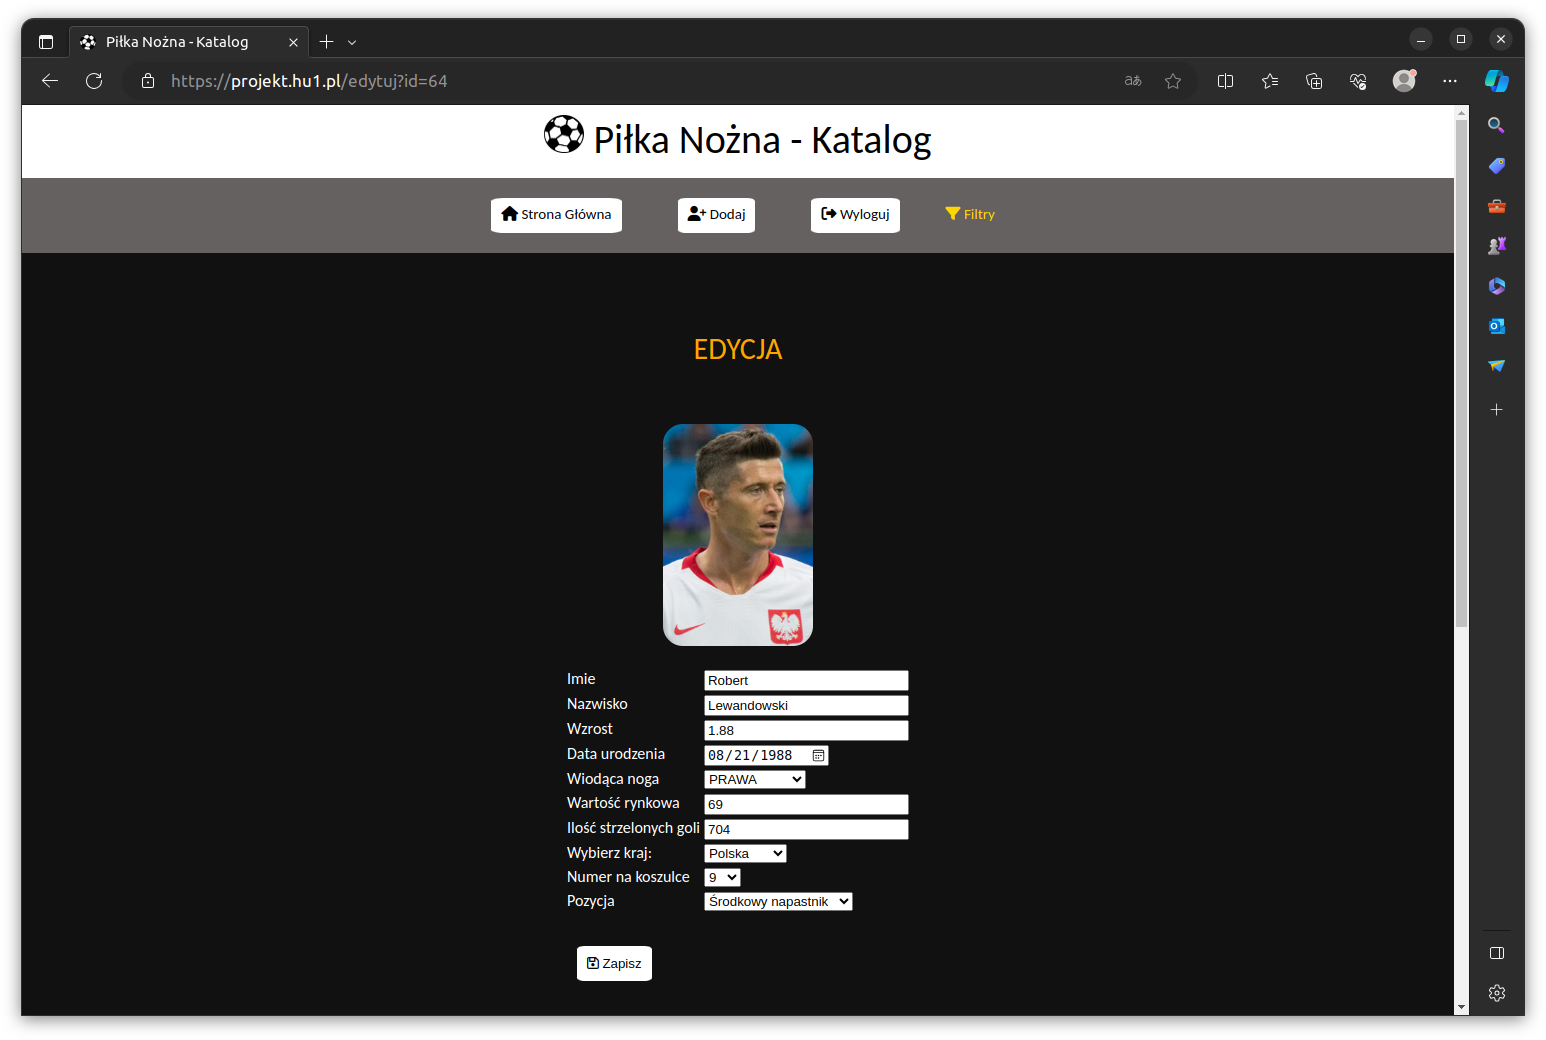
\includegraphics[width=0.6\textwidth]{przewodnik/edycja.png}
                        \caption{Panel służący do edycji informacji na temat piłkarza}                
                    \end{figure}
 